\documentclass[twoside,openright,a4paper,12pt]{memoir}
\usepackage[utf8]{inputenc}
\usepackage{lmodern}
\usepackage[sc]{mathpazo}
\linespread{1.05}
\usepackage[T1]{fontenc}
\usepackage[backend=biber,citestyle=authoryear-comp,hyperref=true]{biblatex}
\usepackage{todonotes}
\usepackage{graphicx}
\usepackage{tikz}
\usetikzlibrary{decorations.pathmorphing,backgrounds,positioning,fit}
\usepackage{gensymb}
\usepackage{amsfonts}
\usepackage{amsthm}
\usepackage[version=3,arrows=pgf]{mhchem}
\usepackage{listings}
\usepackage[
  bookmarks,pdfborder={0,0,0}, colorlinks=true, linkcolor=blue,urlcolor=blue,
  citecolor=blue
]{hyperref}
\usepackage{cleveref}

\theoremstyle{definition}
\newtheorem{defn}{Definition}

\lstset{
  language=[ISO]C++,
  breaklines=true,
  basicstyle=\ttfamily\footnotesize,
  numbers=left,
  numberstyle=\tiny\color{gray},
  stepnumber=2
}

\lstdefinelanguage{opencl}[ISO]{C++} {
  morekeywords={
    float2,float3,float4,int2,int3,int4,uint,uin2,uint3,uint4,
    image2d_t,
    __kernel,__read_only,__local,__global,
    async_work_group_copy, async_work_group_strided_copy, wait_group_events,prefetch,
    clamp,degrees,max,min,mix,radians,sign,smoothstep,step,
    mem_fence,read_mem_fence,write_mem_fence,
    cross,dot,distance,length,normalize,fast_distance,fast_length,fast_normalize,
    read_imagef,read_imagei, read_imageui,read_imageh,write_imageh,write_imagef,write_imagei,write_imageui,get_image_width,get_image_height,get_image_depth,get_image_channel_data_type,get_image_channel_order,get_image_dim,
    abs,abs_diff,add_sat,hadd,rhadd,clz,clamp,mad_hi,mad24,mad_sat,mul_hi,mul24,rotate,sub_sat,upsample,
    get_global_id,
  }
}

\pagestyle{ruled}
\setcounter{tocdepth}{3}

\addbibresource{bibliography.bib}
\addbibresource{chapters/karstification/karstification.bib}
\addbibresource{chapters/opencl/opencl.bib}
\addbibresource{chapters/marchingcubes/marchingcubes.bib}
\addbibresource{chapters/project/project.bib}

\begin{document}
\title{MODELLING SYSTEM OF KARST CAVES FOR COMPUTER GRAPHICS}
\author{Miłosz Kosobucki}

\maketitle
\listoftodos
\newpage

\begin{center}
  \LARGE{Oświadczenie}
\end{center}

Ja, niżej podpisany \textbf{Miłosz Kosobucki} student Wydziału
Matematyki i Informatyki Uniwersytetu im. Adama Mickiewicza w Poznaniu
oświadczam, że przedkładaną pracę dyplomową pt.:

\textbf{Modelling system of karst caves for computer graphics}

napisałem samodzielnie. Oznacza to, że przy pisaniu pracy, poza niezbędnymi
konsultacjami, nie korzystałem z pomocy innych osób, a w szczególności nie
zlecałem opracowania rozprawy lub jej części innym osobom, ani nie
odpisywałem tej rozprawy lub jej części od innych osób.

Oświadczam również, że egzemplarz pracy dyplomowej w formie wydruku
komputerowego jest zgodny z egzemplarzem pracy dyplomowej w formie
elektronicznej.

Jednocześnie przyjmuję do wiadomości, że gdyby powyższe oświadczenie
okazało się nieprawdziwe, decyzja o wydaniu mi dyplomu zostanie cofnięta.

\newcommand{\kropki}[2]{%
  \vbox{%
    \hbox to #1{\dotfill}%
    \vspace{4pt}%
    \hbox to #1{\hss #2\hss}%
  }
}
\vspace{1cm}
\hbox to \textwidth{%
  \hfil
  \kropki{4cm}{data}%
  \hfil\hfil
  \kropki{4cm}{podpis}%
  \hfil
}% \hfil = \hskip 0pt plus 1fil
% \hss = \hskip 0pt plus 1fil minus 1fil
% \hfilneg = \hskip 0pt plus -1fil
\newpage

\begingroup
\footnotesize
\setlength{\parindent}{0pt}
\setlength{\parskip}{\baselineskip}
\copyright 2011 --- 2013 Miłosz Kosobucki \\
All rights reserved
\endgroup

\tableofcontents

\chapter{Introduction}

%This chapter describes motivations behind the development of the thesis. It
%first briefly describes the challenges that arise with ever-increasing capacity
%of computer hardware, that enables nearly photorealistic quality in real-time graphics, but
%at the same time requires enormous amounts of artistic content like models and textures. Procedural
%generation helps to overcome this problem by the usage of parametrized
%algorithms that take limited user input and generate content usually by means
%of randomization or simulation of physical phenomena.
%
%One of such types of content, that may be desirable to generate is a karst cave.
%This geological structure may be an interesting setting for a movie scene or a
%computer game level. At the same time, it is a very complex structure
%that may be time-consuming to model by hand in a way that is both aesthetically
%pleasing and, at least partially, physically correct.

%\section{Advancement of graphics-generation hardware}

%Capabilities of modern computer graphics hardware enables it to


Karst formations are ubiquitous in every continent of Earth. It's estimated that
about 25\% of Earth population depends on drinking water obtained from karst
aquifers \parencite{ford2007karst}. With such profound infulence on human race,
it is essential to know how these geological structures evolve and how they may
react to human activity.

Various simulation models were developed that try to predict how karst aquifers
evolve in time, and how they react to changes in environment. These models are
implemented in computer software and represent simulated karst structure as
net of fractures.

These tools, being aimed at speleogenesis experts, present results of
calculations with simple plots. Programming project of this thesis called \emph{karstgen} provides
solution for richer presentation of geometric structure of modelled karst
structure. It can take input data in format that is similar to formats used by
simulation software for results and generate triangle mesh in two file formats,
of which one is simple and popular textual file format supported by most
three--dimensional modelling software. Presentation in such program may be
beneficial for better understanding of data or for later usage in e.g. video
games.

Since karst evolution models usually simulate large datasets karstgen uses
GPU acceleration to speed--up mesh generation process.

\pagebreak
\section{Structure of the thesis}

Below is overview of each chapter along with description how it contributes to
the thesis.
\begin{description}
  \item[Chapter 2 -- Karst and karstification process] \hfill \\
    This chapter introduces basic definitions related to karst landscape forms
    used later in the work. Karstification process is presented with basic
    overview of chemical reactions that drive it. Information contained in this
    chapter provides rationale for the shape of karst evolution simulation
    models presented in subsequent chapters.
  \item[Chapter 3 -- Related work] \hfill \\
    References to various works relevant to the subject are presented here.
    Brief overview of karst evolution models is presented which explains some
    of the design decisions taken in the programming project.

    Several works related to rendering, rather than simulating, caved terrains
    are also described.
\end{description}


\chapter{Karst and karstification process}
\section{Introduction}
This chapter will briefly describe karst and processes that govern the
development of karts caves.
\todo{Expand when chapter finished}
\section{Basics}

\subsection{Definitions}
\emph{Karstification} is not a strictly defined term. Depending on context it may
mean all forms of corrosion of soluble rocks or it may encompass whole range of
processes that lead to devolopment of karst formations.

Usually karstification means a landscape forming process that consists of dissolution
of various kinds of bedrock. The most common kinds of solutes are limestone,
dolomite, and gypsum \parencite{karstglossary}. However, given right conditions
even some weathering-resistant rocks like quartzite may be subject to 
karstification \parencite{migon2010}\todo{Check reference}.

Although chemical dissolution is the main driving force behind karstification,
mechanical forces may also play a role in the final looks of karst landscape.
That's why sometimes, all these forces together are put under the umbrella term
of karstification.

\emph{Karst} is a terrain formation developed throught means of
\emph{karstification}. The origin of the term is a German form of Slavic word
kras or krš meaning bleak, waterless place.

\subsection{Elements of karst landscape}

Karstification process may produce very interesting and varied landscape. Some
of the prominent elements of karst landscapes are:

\begin{description}
  \item[Sinkholes]
  \item[Caves]
  \item[Resurgences] places where water that went into the aquifer is 
    reemerging to the surface
  \item[Disappearing streams]
  \item[Tunnels]
  \item[Shafts]
\end{description}

\begin{figure}
  \centerline{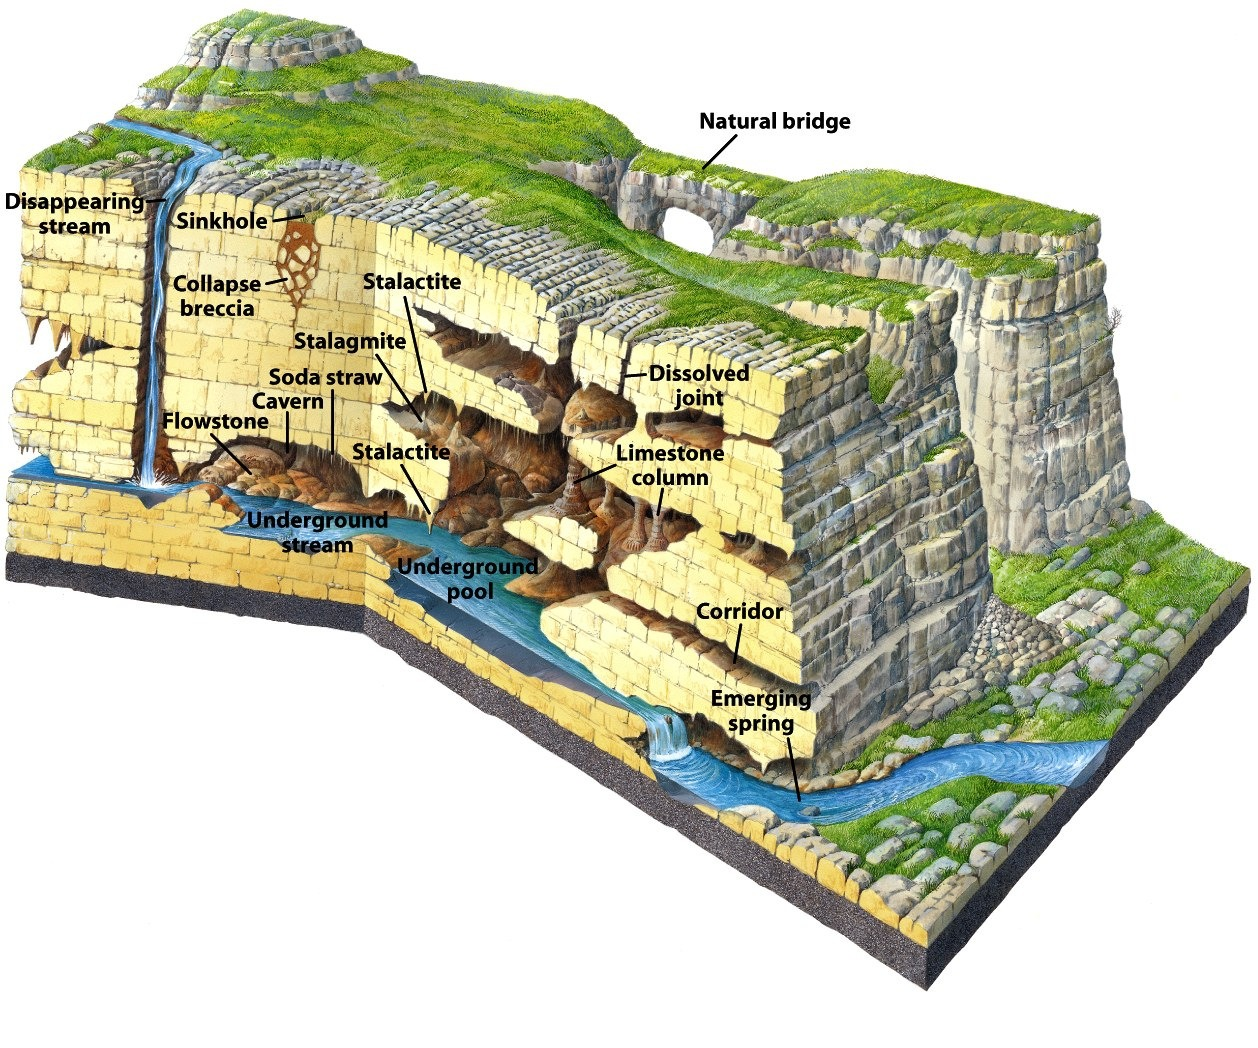
\includegraphics[width=480px]{chapters/karstification/karst_landscape.jpg}}
  \caption{Karst landscape showing various features of karst aquifers.
    Figure from \cite{marshak2006}}
\end{figure}

\todo{Write about karst formations}

\section{Overview of karstification process}

Most important factor in karstification process is flow of solvent throught an
underground aquifer. Since bedrock is subject to geological processes, a
net of fractures of varying diameter and shape is present in it. Water that flows
through this kind of net reacts with rock in ways described later.

The inflow of water to the system may come from precipation, rivers or lakes.

Water that flows through the aquifer reacts chemically with walls of the fractures
widening them through dissolution.

There are also cases of ground formation resulting from human activity.
Although not truly a karst process, a sinkhole that opened in 2010 in city of
Guatemala was a result of combination of loose ground made of volcanic ash and
inadequate draining system, that couldn't dissipate large amounts of water
brought by tropical storm Agatha \parencite{times2010}.

\section{Limestone dissolution}

Chemical reactions that take place during the karstification process will be
shown for limestone aquifers. Following description is taken form \cite{dreybrodt2002}
which is based on \cite{plummer1978}.

As the rain passes throught the atmosphere, it's picking up carbon dioxide that
gets dissolved in water. During this dissolution, small amounts of carbonic acid
are produced:

\ce{H2O + CO2 -> H2CO3} \todo{describe reactions}

\ce{H2O + CaCO3 <-> Ca^2 + CO3^{2-} + H2O}

\section{Formation of speleothems}

\chapter{Related work}
\label{chap:related}

This chapter presents basics of modelling of processes governing evolution of
karst aquifers. This description will provide basis for the data formats
used in programming project. Some visualisation techniques used previously for
caved terrains will also be presented.

\section{Modelling karst aquifers}

As karst aquifers contain network of fractures (see \autoref{chap:karstification})
a simulation of flow and chemical reactions in single fracture is the basic
building block of presented models.

These fractures are connected to form larger, two or three--dimensional networks,
that represent whole conduits.

First attempts to describe processes taking place during evolution of karst
aquifers with numerical models took place in early 1980's \parencite[p. 3]{hiller2013}.
\Cite{Buhmann1985189} developed numerical model for ternary chemical system
(\cee{CaCO3}--\cee{CO2}--\cee{H2O}) in open systems (where \cee{CO2} is exchanged
with atmosphere) and for closed ones \parencite{Buhmann1985109}.

\subsection{Single fracture simulation}

With these dissolution models in place several models of single conduit were
presented \parencite[pp. 4]{hiller2013}.

Single fracture is modelled as a circular conduit in the intersection
of fissure and bedding plane \parencite{Kaufmann200962} or as a space between
two parallel walls of rock separated by aperture width \parencite{dreybrodt2002}.

\subsection{Two--dimensional simulations}

Single conduit one--dimensional models were later expanded into second dimension
by combining set of conduits into a connected network \parencite[pp. 4--5]{hiller2013}.
In such networks, fractures are organized into uniform, regular structure.

\subsection{Three--dimensional simulations}

With more powerful computational resources researchers started research on
three--dimensional models that could finally provide insight into evolution
of real--life karst aquifers. Such models were proposed by
\cites{annable2003}{WRCR:WRCR9525}{Kaufmann2010241}.

Work by \cite{hiller2013} summarizes current state of three--dimensional models.
His thesis contains overview of modelling techniques and approaches. Simulation
of real--live karst aquifer near dam--site is presented that matches
observations. This shows validity of proposed models.

\section{Visualisation techniques}

Rendering techniques that touched the issue of cave rendering never tried to
provide both physical accuracy and visually appealing graphics.

In \cite{gpugems3ch01} a method for rendering procedural terrains is described
that in some circumstances can generate caves. Similar to this work, presented
method uses Marching Cubes algorithm (see \autoref{chap:marchingcubes})
implemented on GPU (albeit in shaders, and not with any GPGPU solution) and
carefully crafted density functions based on noise sampling.

\Cite{forstmann2005} proposed method of on--the--fly rendering of procedural
terrains that may also contain caves. It uses hierarchy of nested clip--boxes
for LOD\footnote{Level of detail} calculation to reduce workload of the GPU.

\chapter{OpenCL heterogenous programming platform}

\chapter{Isosurface extraction with Marching Cubes}
\label{chap:marchingcubes}

This chapter will present a method of isosurface extraction that is later used
in the programming project. First, basic definitions will be established and
rationale for generating graphics with volumetric data will be discussed.
Next, brief history and high level overview of Marching Cubes will be presented.
Technical details will follow with description of implementation on highly
parallel GPGPU systems with OpenCL.

\section{Definitions}

\begin{defn}[Density function]
\label{def:density function}
Scalar function
$\mathbb{R}^3\rightarrow\mathbb{R}$ or $\mathbb{R}^2\rightarrow\mathbb{R}$
that defines value of some magnitude in a continuous space. An example of such
function in 3D space is temperature defined in each point in the space. Height
on a flat map on the other hand is a density function in 2D space.
\end{defn}

\begin{defn}[Isosurface]
Surface in three-dimensional space that consists of points that have certain
value of \emph{density function}.
\end{defn}

\begin{defn}[Isovalue]
Certain value of density function which will be considered the surface. Points
in domain which density function value is below this value are considered to
lie below the surface and points which density function value is above this
value are considered to lie above the surface. Points which density function
value is equal to the isovalue are considered to lie exactly on the isosurface.
\end{defn}

\section{Rationale for isosurface rendering}

There are many applications which yield data as a density function. Some of them
are listed below:
\begin{description}
	\item[CT\footnotemark scan.]\footnotetext{Computer Tomography}
		Result of such scan is a set of 2D slices with each slice
		consisting of array of scalar values \parencite{Lorensen:1987:MCH:37402.37422}.
	\item[Weather data]
		Weather data, especially coming from weather models consists of
		scalar values of various parameters (temperature, humidity, etc.)
		on earth's surface
	\item[Arbitrary mathematical function]
		It's often desirable to visualise mathematical function with
		multiple parameters on 2D and 3D plots. For example for
		educational purposes.
	\item[Procedural models]
		Surfaces expressed by density function may be a source of
		visually interesting models that could be hard to model by hand.
\end{description}

Interactive presentation of such data may be very helpful while working with
these applications. Ability to rotate, zoom and scale such surfaces is
beneficial to understanding the data since human sight apparatus is naturally
well equipped to process 3D objects and images.

\section{Marching Cubes algorithm overview}
\subsection{History \parencite{mchist}}
Marching Cubes algorithm was invented in 1984 by William E. Lorensen and Harvey
E. Cline. While being employed by General Electric they attended a seminar by
GE's Medical Systems Business Group employee Carl Crawford. Mr Crawford
described capabilities of the upcoming rendering engine called \emph{Graphicon},
that rendered using polygons. He also challenged seminar attendees to find
interesting usages for the device. Within a day Lorenson and Cline devised an
algorithm that read volumetric medical data (essentially a density function) and
produced triangle mesh representing isosurface.

General Electric submitted a patent application for the algorithm on
June~5, 1985, which was granted on December~1, 1987 \parencite{mcpatent}.

Partly due to existence of this patent, another algorithm called
\emph{Marching Tetrahedra} was invented to give graphics community another
method of isosurface extraction, that is not encumbered by patents.
\emph{Marching Tetrahedra} also solves some ambiguities that are present in
\emph{Marching Cubes}.

Patent on \emph{Marching Cubes} algorithm expired in 2005.

\subsection{Algorithm description \parencite{Lorensen:1987:MCH:37402.37422}}
\label{sec:mcdesc}

Marching cubes algorithm divides space on which it operates into a discrete
lattice of cubes (interchangeably called \emph{voxels}). For each cube, density
function value is retrieved for each vertex of the cube. Density function may be
calculated from the position of the vertex on the fly if it's defined as a
mathematical function, or it may be extracted from some external volumetric data
source (e.g. result of CT scan).

Next, for each vertex of the cube it's determined whether value at its position
is larger or smaller than requested isovalue. If the value on the vertex is
smaller vertex is below the surface. Otherwise it's above it.

Being above or below the surface will be called the \emph{sign} of the vertex.
If vertices on the ends of given cube's edge are of different signes, than it's
certain that the surface crosses the edge.

For each cube, there are $2^8=256$ possible combinations of sings of the
vertices. Combination of the cube is called an \emph{index} of this cube.

When the index of the cube is known, pre-generated LUTs\footnote{Look-Up Tables}
are consulted to determine how many polygons and in what configuration should be
emitted for this cube.

Original version of Marching Cubes algorithm divides all 256 possible
combinations of vertices into 15 cases. These cases are presented in
\autoref{fig:mccases}. Remaining combinations are derivatives of these cases
(symmetries, rotations, and complimentary cases).

Process is repeated for all cubes in the lattice and emitted polygons (possibly
with normal vectors for lighting) are the output of the algorithm.

\begin{figure}
  \centerline{
    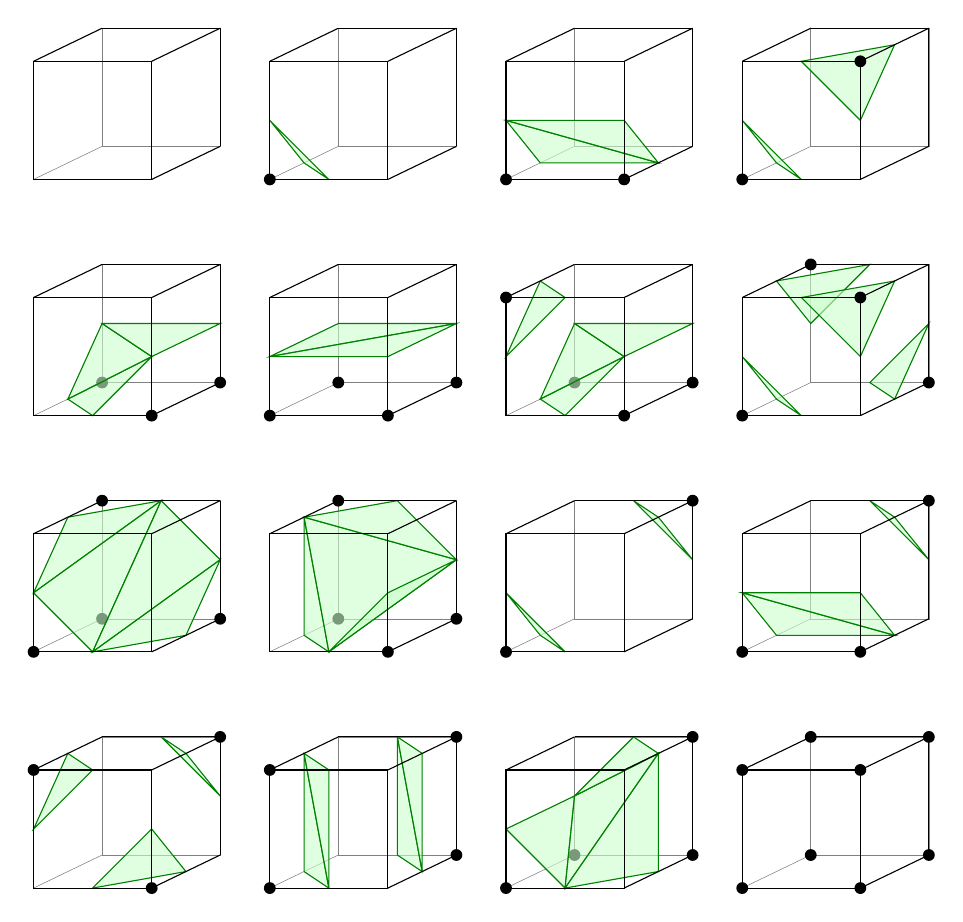
\begin{tikzpicture}[z={(-0.58cm,-0.28cm)}, scale=1.5]
      \tikzstyle{vertexfill} = [fill=green!20, fill opacity=0.6, draw=green!50!black]

  \def\cubeback{
    \draw[gray,very thin] +(0,0,-1) rectangle +(1,1,-1);
    \draw[gray,very thin] +(0,0,0) -- +(0,0,-1);
  }
  \def\cubefront{
    \draw +(1,0,-1) -- +(1,1,-1);
    \draw +(0,1,-1) -- +(1,1,-1);
    \draw +(0,0,0) rectangle +(1,1,0);
    \draw +(0,1,0) -- +(0,1,-1);
    \draw +(1,0,0) -- +(1,0,-1);
    \draw +(1,1,0) -- +(1,1,-1);
  }

  \begin{scope}[shift={(0,0)}]
    \cubeback
    \cubefront
  \end{scope}

  \begin{scope}[shift={(2,0)}]
    \cubeback
    \filldraw[vertexfill]
      (0,0.5,0) -- (0,0,-0.5) -- (0.5,0,0) -- cycle;
    \fill (0,0) circle (0.05);
    \cubefront
  \end{scope}

  \begin{scope}[shift={(4,0)}]
    \cubeback
    \filldraw[vertexfill]
      (0,0,-0.5) -- (0,0.5,0) -- (1,0,-0.5) -- cycle;
    \filldraw[vertexfill]
      (0,0.5,0) -- (1,0.5,0) -- (1,0,-0.5) -- cycle;
    \fill (0,0) circle (0.05);
    \fill (1,0) circle (0.05);
    \cubefront
  \end{scope}

  \begin{scope}[shift={(6,0)}]
    \cubeback
    \filldraw[vertexfill]
      (0,0.5,0) -- (0,0,-0.5) -- (0.5,0,0) -- cycle;
    \filldraw[vertexfill]
      (1,0.5,0) -- (1,1,-0.5) -- (0.5,1,0) -- cycle;
    \fill (0,0) circle (0.05);
    \fill (1,1) circle (0.05);
    \cubefront
  \end{scope}
  \begin{scope}[shift={(0,-2)}]
    \cubeback
    \fill (0,0,-1) circle (0.05);
    \filldraw[vertexfill]
      (0,0,-0.5) -- (0.5,0,0) -- (1,0.5,0) -- cycle;
    \filldraw[vertexfill]
      (0,0,-0.5) -- (0,0.5,-1) -- (1,0.5,0) -- cycle;
    \filldraw[vertexfill]
      (1,0.5,0) -- (1,0.5,-1) -- (0,0.5,-1) -- cycle;
    
    \fill (1,0) circle (0.05);
    \fill (1,0,-1) circle (0.05);
    \cubefront
  \end{scope}
  \begin{scope}[shift={(2,-2)}]
    \cubeback
    \filldraw[vertexfill]
      (0,0.5,0) -- (1,0.5,-1) -- (0,0.5,-1) -- cycle;
    \filldraw[vertexfill]
      (0,0.5,0) -- (1,0.5,0) -- (1,0.5,-1) -- cycle;

    \fill (0,0) circle (0.05);
    \fill (1,0) circle (0.05);
    \fill (1,0,-1) circle (0.05);
    \fill (0,0,-1) circle (0.05);
    \cubefront
  \end{scope}
  \begin{scope}[shift={(4,-2)}]
    \cubeback
    \fill (0,0,-1) circle (0.05);
    \filldraw[vertexfill]
      (0,0.5,0) -- (0.5,1,0) -- (0,1,-0.5) -- cycle;
    \filldraw[vertexfill]
      (0,0,-0.5) -- (0.5,0,0) -- (1,0.5,0) -- cycle;
    \filldraw[vertexfill]
      (0,0,-0.5) -- (0,0.5,-1) -- (1,0.5,0) -- cycle;
    \filldraw[vertexfill]
      (1,0.5,0) -- (1,0.5,-1) -- (0,0.5,-1) -- cycle;

    \fill (0,1,0) circle (0.05);
    \fill (1,0) circle (0.05);
    \fill (1,0,-1) circle (0.05);
    \cubefront
  \end{scope}
  \begin{scope}[shift={(6,-2)}]
    \cubeback
    \fill (0,1,-1) circle (0.05);
    \fill (1,0,-1) circle (0.05);
    \filldraw[vertexfill]
      (0,1,-0.5) -- (0,0.5,-1) -- (0.5,1,-1) -- cycle;
    \filldraw[vertexfill]
      (0,0.5,0) -- (0,0,-0.5) -- (0.5,0,0) -- cycle;
    \filldraw[vertexfill]
      (1,0.5,0) -- (1,1,-0.5) -- (0.5,1,0) -- cycle;
    \filldraw[vertexfill]
      (1,0,-0.5) -- (1,0.5,-1) -- (0.5,0,-1) -- cycle;

    \fill (1,1) circle (0.05);
    \fill (0,0) circle (0.05);
    \cubefront
  \end{scope}
  \begin{scope}[shift={(0,-4)}]
    \cubeback
    \fill (0,1,-1) circle (0.05);
    \fill (0,0,-1) circle (0.05);
    \fill (1,0,-1) circle (0.05);
    \filldraw[vertexfill]
      (0,0.5,0) -- (0.5,1,-1) -- (0,1,-0.5) -- cycle;
    \filldraw[vertexfill]
      (0,0.5,0) -- (0.5,0,0) -- (0.5,1,-1) -- cycle;
    \filldraw[vertexfill]
      (0.5,0,0) -- (1,0.5,-1) -- (0.5,1,-1) -- cycle;
    \filldraw[vertexfill]
      (0.5,0,0) -- (1,0,-0.5) -- (1,0.5,-1) -- cycle;
    \fill (0,0) circle (0.05);
    \cubefront
  \end{scope}
  \begin{scope}[shift={(2,-4)}]
    \cubeback
    \fill (0,0,-1) circle (0.05);
    \fill (1,0,-1) circle (0.05);
    \fill (0,1,-1) circle (0.05);

    \filldraw[vertexfill]
      (0,0,-0.5) -- (0.5,0,0) -- (0,1,-0.5) -- cycle;
    \filldraw[vertexfill]
      (0.5,0,0) -- (1,0.5,-1) -- (0,1,-0.5) -- cycle;
    \filldraw[vertexfill]
      (0.5,0,0) -- (1,0.5,0) -- (1,0.5,-1) -- cycle;
    \filldraw[vertexfill]
      (0,1,-0.5) -- (1,0.5,-1) -- (0.5,1,-1) -- cycle;

    \fill (1,0) circle (0.05);
    \cubefront
  \end{scope}
  \begin{scope}[shift={(4,-4)}]
    \cubeback
    \fill (1,1,-1) circle (0.05);
    \filldraw[vertexfill]
      (0,0.5,0) -- (0,0,-0.5) -- (0.5,0,0) -- cycle;
    \filldraw[vertexfill]
      (1,1,-0.5) -- (1,0.5,-1) -- (0.5,1,-1) -- cycle;
    \fill (0,0) circle (0.05);
    \cubefront
  \end{scope}
  \begin{scope}[shift={(6,-4)}]
    \cubeback
    \fill (1,1,-1) circle (0.05);
    \filldraw[vertexfill]
      (1,1,-0.5) -- (1,0.5,-1) -- (0.5,1,-1) -- cycle;
    \filldraw[vertexfill]
      (0,0,-0.5) -- (0,0.5,0) -- (1,0,-0.5) -- cycle;
    \filldraw[vertexfill]
      (0,0.5,0) -- (1,0.5,0) -- (1,0,-0.5) -- cycle;
    \fill (0,0) circle (0.05);
    \fill (1,0) circle (0.05);
    \cubefront
  \end{scope}
  \begin{scope}[shift={(0,-6)}]
    \cubeback
    \fill (1,1,-1) circle (0.05);
    \filldraw[vertexfill]
      (1,1,-0.5) -- (1,0.5,-1) -- (0.5,1,-1) -- cycle;
    \filldraw[vertexfill]
      (0,0.5,0) -- (0.5,1,0) -- (0,1,-0.5) -- cycle;
    \filldraw[vertexfill]
      (0.5,0,0) -- (1,0,-0.5) -- (1,0.5,0) -- cycle;

    \fill (1,0,0) circle (0.05);
    \fill (0,1,0) circle (0.05);
    \cubefront
  \end{scope}
  \begin{scope}[shift={(2,-6)}]
    \cubeback
    \fill (1,1,-1) circle (0.05);
    \fill (1,0,-1) circle (0.05);

    \filldraw[vertexfill]
      (0,0,-0.5) -- (0.5,0,0) -- (0,1,-0.5) -- cycle;
    \filldraw[vertexfill]
      (0,1,-0.5) -- (0.5,0,0) -- (0.5,1,0) --  cycle;
    \filldraw[vertexfill]
      (1,0,-0.5) -- (0.5,1,-1) -- (0.5,0,-1) -- cycle;
    \filldraw[vertexfill]
      (1,0,-0.5) -- (1,1,-0.5) -- (0.5,1,-1) -- cycle;

    \fill (0,0,0) circle (0.05);
    \fill (0,1,0) circle (0.05);
    \cubefront
  \end{scope}
  \begin{scope}[shift={(4,-6)}]
    \cubeback
    \fill (0,0,-1) circle (0.05);
    \fill (1,1,-1) circle (0.05);
    \fill (1,0,-1) circle (0.05);

    \filldraw[vertexfill]
      (0,0.5,0) -- (0.5,0,0) -- (0,0.5,-1) -- cycle;
    \filldraw[vertexfill]
      (0.5,0,0) -- (1,1,-0.5) -- (0,0.5,-1) -- cycle;
    \filldraw[vertexfill]
      (0.5,0,0) -- (1,0,-0.5) -- (1,1,-0.5) -- cycle;
    \filldraw[vertexfill]
      (1,1,-0.5) -- (0.5,1,-1) -- (0,0.5,-1) -- cycle;

    \fill (0,0,0) circle (0.05);
    \cubefront
  \end{scope}
  \begin{scope}[shift={(6,-6)}]
    \cubeback
    \fill (0,0,0) circle (0.05);
    \fill (0,0,-1) circle (0.05);
    \fill (0,1,0) circle (0.05);
    \fill (0,1,-1) circle (0.05);
    \fill (1,0,0) circle (0.05);
    \fill (1,0,-1) circle (0.05);
    \fill (1,1,0) circle (0.05);
    \fill (1,1,-1) circle (0.05);
    \cubefront
  \end{scope}

    \end{tikzpicture}
  }
  \caption{
    All cases in traditional Marching cubes algorithm. Vertices with density
    function above threshold value have black circles on them. Symmetries,
    rotations, and complementary cases (with exception of cases 0 and 255) were
    omitted for brevity.
  }
  \label{fig:mccases}
\end{figure}

\subsubsection{Cube indexing}

Operation on a single cube begins with evaluating density function on each
vertex of the cube.

Index of the vertex is calculated through operation described below
\autoref{fig:mcnumbering}.

\begin{figure}
  \centerline{
   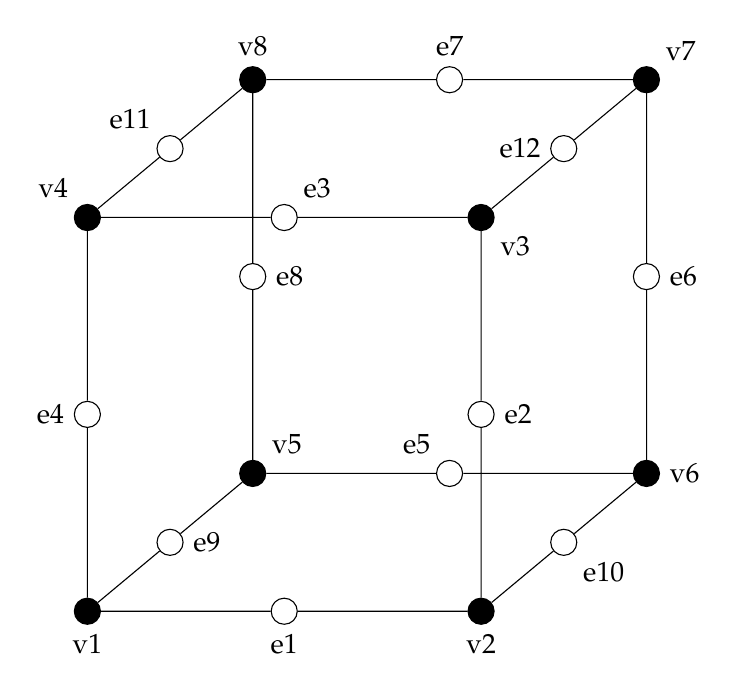
\begin{tikzpicture}[
  z={(-0.42cm,-0.35cm)}, scale=2.5,
  vert/.style={circle,draw=black,fill=black},
  edge/.style={circle,draw=black,fill=white}
]
 
  \node at (0,0,0) [vert,label=below:v1] (v1) {};
  \node at (1,0,0) [edge,label=below:e1] (e1) {};
  \node at (2,0,0) [vert,label=below:v2] (v2) {};
  \node at (2,1,0) [edge,label=right:e2] (e2) {};
  \node at (2,2,0) [vert,label=south east:v3] (v3) {};
  \node at (1,2,0) [edge,label=north east:e3] (e3) {};
  \node at (0,2,0) [vert,label=north west:v4] (v4) {};
  \node at (0,1,0) [edge,label=left:e4] (e4) {};
  \node at (0,0,-2) [vert,label=north east:v5] (v5) {};
  \node at (1,0,-2) [edge,label=north west:e5] (e5) {};
  \node at (2,0,-2) [vert,label=right:v6] (v6) {};
  \node at (2,1,-2) [edge,label=right:e6] (e6) {};
  \node at (2,2,-2) [vert,label=north east:v7] (v7) {};
  \node at (1,2,-2) [edge,label=above:e7] (e7) {};
  \node at (0,2,-2) [vert,label=above:v8] (v8) {};
  \node at (0,1,-2) [edge,label=right:e8] (e8) {};
  \node at (0,0,-1) [edge,label=right:e9] (e9) {};
  \node at (2,0,-1) [edge,label=south east:e10] (e10) {};
  \node at (2,2,-1) [edge,label=left:e12] (e12) {};
  \node at (0,2,-1) [edge,label=north west:e11] (e11) {};

  \draw
    (v1) -- (e1) -- (v2) -- (e2) -- (v3) -- (e3) -- (v4) -- (e4) -- (v1)
    (v5) -- (e5) -- (v6) -- (e6) -- (v7) -- (e7) -- (v8) -- (e8) -- (v5)
    (v1) -- (e9) -- (v5)
    (v2) -- (e10) -- (v6)
    (v4) -- (e11) -- (v8)
    (v3) -- (e12) -- (v7);
\end{tikzpicture}

  }
  \caption{
    Numbering of vertices and edges in Marching Cubes. Cube index is
    derived by concatenation of bits \texttt{index = v8|v7|v6|v5|v4|v3|v2|v1}
    where each \texttt{vi} is logical result (0 or 1) of operation of comparing
    density function value at \emph{i}-th vertex with threshold value
    (\texttt{value(i) > threshold}).
  }
  \label{fig:mcnumbering}
\end{figure}

\subsubsection{Emitting polygons}
\label{sec:mcemitting}

When index of the cube is known, LUT is consulted that maps index to list of
edges on which vertex in given cube must be emitted.

\begin{lstlisting}[caption={Index to edge list LUT. Notice that for indices 0
and 255 no geometry is emitted}]
unsigned char mcTriangleTable[256][16] = {
        {255, 255, 255, 255, 255, 255, 255, 255, 255, 255, 255, 255, 255, 255, 255, 255},
        {0, 8, 3, 255, 255, 255, 255, 255, 255, 255, 255, 255, 255, 255, 255, 255},
        ...
        {0, 3, 8, 255, 255, 255, 255, 255, 255, 255, 255, 255, 255, 255, 255, 255},
        {255, 255, 255, 255, 255, 255, 255, 255, 255, 255, 255, 255, 255, 255, 255, 255}
};
\end{lstlisting}

For each edge on the list vertex is emitted between its two ends in place
proportional to the linear interpolation of density function at the vertices.

Each three vertices form a polygon. In the listing above, value 255 marks an end
of the list for given index.

Next, each polygon is saved in a list for later usage, or directly fed to
rendering device.

\section{Implementation on GPU with OpenCL}
\label{sec:mcgpu}
Following implementation is based on example code from NVIDIA CUDA SDK
example\footnote{\url{http://docs.nvidia.com/cuda/cuda-samples/index.html\#marching-cubes-isosurfaces}}.

As described in \autoref{sec:mcdesc} each cube is processed by the algorithm
independently. This possibly makes this algorithm a good candidate for massive
parallelization offered by GPGPUs. There are however some obstacles to overcome.

First, LUTs used by the algorithm are obviously too big to fit into registers.
Reading them from global memory would also be problematic, because they are
accessed in a random manner, depending on cube index. Tables could be copied
to local memory for faster access, but the cost of copying for each block could
be substantial.

Another problem is storage of the output. It is not known beforehand how many
polygons will be emitted by each cube. With sequential implementation it isn't a
problem because data generated by each cube may be just appended to single
result array. With many cubes being process at the same time, this approach
will not work.

\subsection{Stages in GPU implementation}
Kernel execution is divided into the following stages:
\todo{insert image with stages diagram}

All operations are performed on cube lattice flattened to 1D array. Each stage
of the execution will be described below.

\subsubsection{Voxel classification}

In this stage, all voxels are classified as to whether they will produce any
geometry or not, and how many vertices is given voxel going to produce.

Results are written to two arrays \texttt{voxelOccupied} which contains 1
if given voxel produces any geometry and 0 otherwise, and
\texttt{voxelVerts} that holds number of vertices produced by this voxel:
\todo{Find out about having single listing with some dialect}
\begin{lstlisting}[language=opencl, numbers=left]
__kernel
void classifyVoxel(
	__global uint *voxelVerts,
	__global uint *voxelOccupied,
	uint4 gridSize,
	float4 voxelSize,
	float isoValue,
	uint numVoxels,
	__read_only image2d_t numVertsTex)
{
	uint i = get_global_id(0);
	float4 cubeValues[8];
	/* Here, values on each vertex of the voxel are inserted into cubeValues array */

	int cubeIndex = getCubeIndex(cubeValues, isoValue);
	uint numVerts = read_imageui(numVertsTex, tableSampler, (int2)(cubeIndex, 0)).x;
	if (i < numVoxels) {
		voxelVerts[i] = numVerts;
		voxelOccupied[i] = (numVerts > 0);
	}
}
\end{lstlisting}
Note that additional lookup table (\texttt{numVertsTex}) that maps cube index to
number of vertices it produces is used. This LUT is accessed as a texture.

Index of the cube is calculated as described in \autoref{fig:mcnumbering}:

\begin{lstlisting}
int getCubeIndex(float4 *cubeValues, float isoValue)
{
	int cubeIndex;
	cubeIndex =  (cubeValues[0].w < isoValue);
	cubeIndex += (cubeValues[1].w < isoValue) << 1;
	cubeIndex += (cubeValues[2].w < isoValue) << 2;
	/*...*/
	cubeIndex += (cubeValues[7].w < isoValue) << 7;
	return cubeIndex;
}
\end{lstlisting}

\subsubsection{Compacting}

\begin{figure}
	\begin{center}
		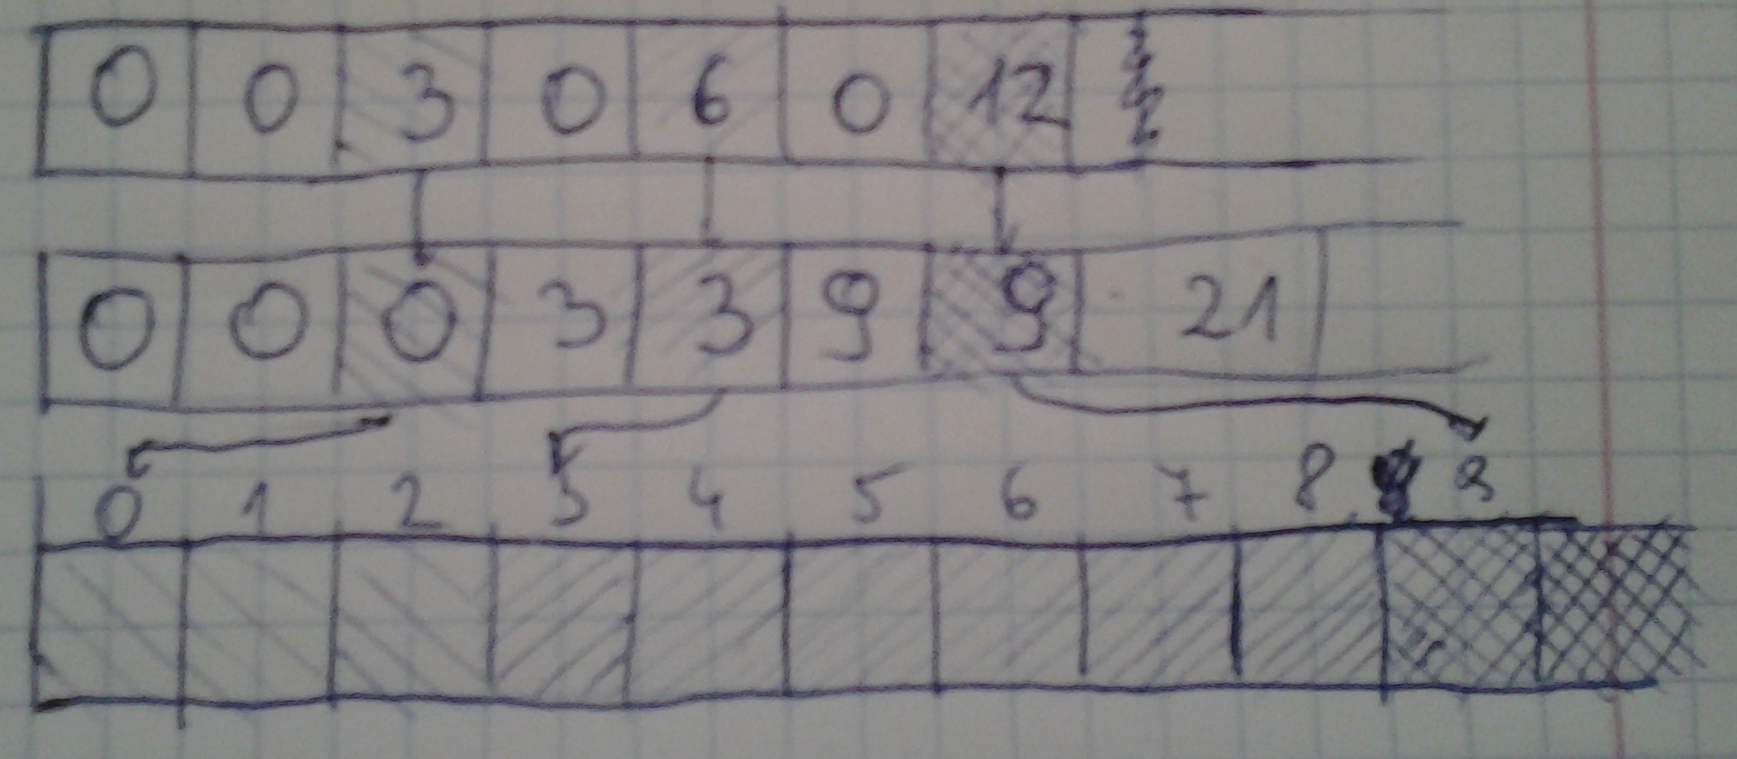
\includegraphics[width=\textwidth]{chapters/marchingcubes/compact.jpg}
	\end{center}
	\caption{Example of compaction procedure. Index of each non empty voxel
		is saved in \texttt{compactedVoxelArray}. Place to which index
		should be stored is read from \texttt{voxelOccupiedScan} array.
	}
	\label{fig:mccompact}
\end{figure}
\todo{replace figure \ref{fig:mccompact} with proper graphics}

To overcome problem highlighted in \autoref{sec:mcgpu} a special compacting
operation is performed on arrays from previous step. First, a prefix-sum array
is computed in parallel on the GPU \footnote{implementation based on \cite{gpugemsscan},
as included in \href{https://developer.nvidia.com/cuda-downloads}{NVIDIA CUDA SDK}}
on \texttt{voxelOccupied} and \texttt{voxelVerts} arrays resulting in
\texttt{voxelOccupiedScan} and \texttt{voxelVertsScan} arrays.

\begin{defn}[Prefix-sum operation \parencite{BlellochTR90}]
operation that takes binary associative operator $\oplus$ with identity $I$ and
an array of $n$ elements $[a_0,a_1,\ldots,a_{n-1}]$ and returns the array
$[I,a_0,(a_0\oplus a_1),\ldots,(a_0\oplus a_1 \oplus \ldots \oplus a_{n-2})]$

This operation is sometimes called \emph{scan} operation.
\end{defn}

By reading the last elements of \texttt{voxelOccupied} and
\texttt{voxelOccupiedScan} and adding them, the number of voxels that will
produce geometry can be obtained. These voxels are called \emph{active voxels}.

Thanks to voxel compaction, the most computation--intensive kernel, i.e.
\texttt{generateTriangles} kernel that generates final geometry can be computed
only for voxels that are not empty. Since in many cases, space on which Marching
cube is working is rather sparse, this approach can bring enormous performance
gains.

Let call the number of active voxels $n$. Compaction kernel creates an array
of length $n$ that will contain indexes of non empty voxels. For illustration of
this process refer to \autoref{fig:mccompact}.

Below is the code that performs the compaction.
\begin{lstlisting}[language=opencl]
__kernel
void compactVoxels(
	__global uint *compactedVoxelArray,
	__global uint *voxelOccupied,
	__global uint *voxelOccupiedScan,
	uint numVoxels
)
{
	uint i = get_global_id(0);
	if(voxelOccupied[i] && (i < numVoxels)) {
		compactedVoxelArray[voxelOccupiedScan[i]] = i;
	}
}
\end{lstlisting}

Scan operation on \texttt{voxelVerts} array gives \texttt{generateTriangles}
kernel offset to the result array where data for given voxel should be written.
For an example refer to \autoref{fig:mcvertscan}.

\begin{figure}[b]
	\begin{center}
		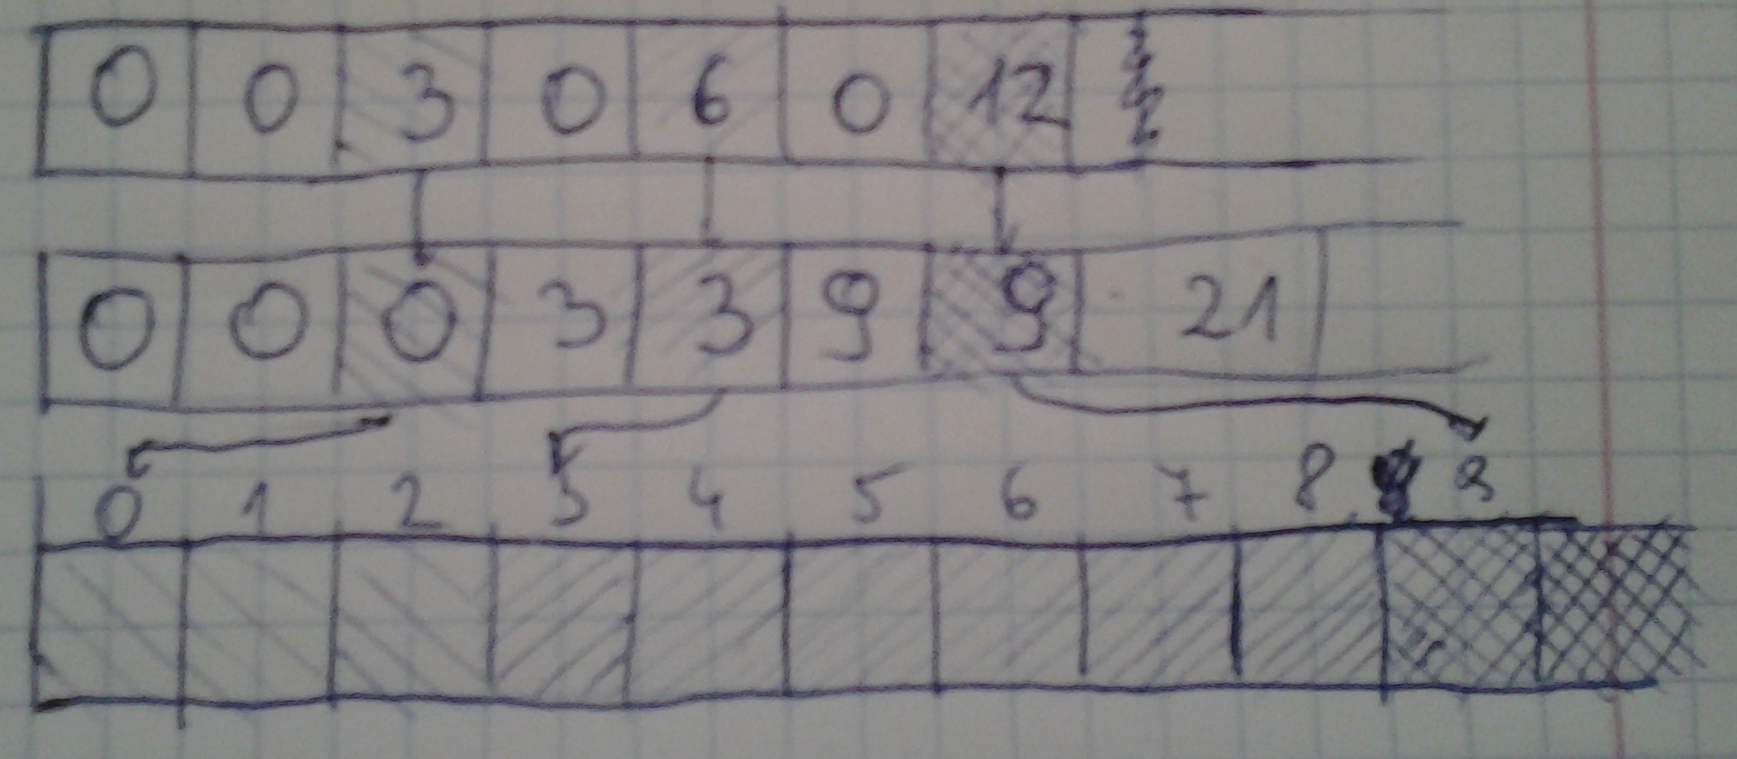
\includegraphics[width=\textwidth]{chapters/marchingcubes/vertscan.jpg}
	\end{center}
	\caption{Scan operation on \texttt{voxelVerts} array gives indexes to
		final result array for every active voxel.
	}
	\label{fig:mcvertscan}
\end{figure}

\subsubsection{Generating trangles}

Triangle generation is handled by \texttt{generateTriangles} kernel. It figures
out the number of voxel it's working on from \texttt{compactedVoxelArray}. Next,
array in local memory is allocated for computing locations of vertices on each
of the 12 edges on the cube.

\begin{lstlisting}
__local float4 vertList[12*NTHREADS];
__local float4 normList[12*NTHREADS];
\end{lstlisting}

Positions are calculated even though certain edges may not have surface border
on them. However, using \texttt{if} statement in kernel in this context would
cause divergence in execution of parallel threads.

From now on, algorithm is the same as in sequential version. List of edges on
which vertices lie is read from LUT mentioned in \autoref{sec:mcemitting}. This
table is accessed as a 2D texture. Agressive caching strategy implemented in
GPUs for texture data access allows the kernel to retrieve the data without
much penalty. Positions of vertices and normals on edges read from LUT are read
from \texttt{vertList} and \texttt{normList} arrays, and are written into result
vertex position and normal arrays on indices read from \texttt{voxelVertsScan}
array.

\chapter{Programming project description}
\label{chap:project}
\section{Introduction}

Programming project of this thesis is a set of command line programs, collectively
called \emph{Karstgen}, that take
the description of karst cave fracture net and generate polygon mesh in
simple and popular Wavefront OBJ textual file format\footnote{\url{http://www.martinreddy.net/gfx/3d/OBJ.spec}}.

Models created this way may be opened in 3D editing program for further editing
and examination.

Karstgen can also create models for \emph{Vorticity} game engine that was created
by the author together with mr Michał Siejak for graphics related courses\footnote{Computer
  Graphics and Visualiation, summer semester 2009/2009 and Group Project, summer
semester 2009/2010} during licenciate studies at Adam Mickiewicz University \todo{check form}in
Poznań.

\section{Architecture}

Karstgen was created with Unix Philosophy in mind \parencite{raymond2003art}.
It is made of two programs named \emph{blobber} and \emph{mcblob} that have
clearly defined reposinsibilities and communicate through simple textual data
format.  Both programs may take input either from files or from standard input
so they can be piped together with shell pipes. Data flow of karstgen is
presented in \autoref{fig:karstgenflow}.
\begin{figure}[ht]
  \begin{center}
    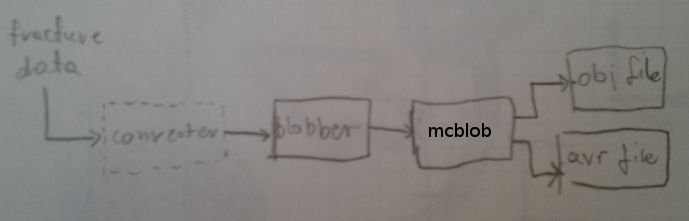
\includegraphics[width=\textwidth]{chapters/project/karstgenflow.jpg}
  \end{center}
  \caption{Data flow of karstgen program. Converter part is required when fracture
  net description is other than expected by blobber.}
  \label{fig:karstgenflow}
\end{figure}
\todo{replace \autoref{fig:karstgenflow} with TikZ graphics}

\subsection{Blobber}
Blobber takes description of a fracture net in a simple textual format and
generates list of metaballs (see \autoref{sub:metaballs}). It can
optionally tilt positions and sizes of metaballs in random but adjustable manner
for more natural--looking results. Blobber also controls quality of the final
geometry. For information about runtime parameters invoke:
\begin{verbatim}
./blobber --help
\end{verbatim}

\subsection{Mcblob}
Output generated by blobber is consumed by program named \emph{mcblob}\footnote{Marching
Cubes from blobs} which is general purpose tool that may be used to
generate geometry from a list of metaballs in 3D space.

\section{Implementation}
\subsection{Metaballs}
Implementation heavily relies on rendering with metaballs. Metaball in 3D space
is a scalar function in the form:
\begin{equation}
  f(x,y,z)=Te^{\frac{B}{R^2}r^2 - B}
  \label{eq:metaball}
\end{equation}
where $r$ is distance from point $(x,y,z)$ to the center of the metaball, $B$ is
,,blobiness'' factor that controls tendency to ,,melt'' with other metaballs, $T$
is isovalue that will be used for rendering and $R$ is the radius of the
metaball if it was isolated from other blobs. This equation is basically a
Gaussian bump centerd in the middle of the metaball.

If more than one metaball is present in the scene, density function (see Definition
\autoref{def:density function})
is in the form:
\begin{equation}
  d(x,y,z) = \sum_{i=0}^{n} f_i(x,y,z)
  \label{eq:metaballdensity}
\end{equation}
where $n$ is the total number of metaballs in the scene and $f_i$ is function~\ref{eq:metaball}
of the $i$-th metaball.

Metaballs were discovered by Jim Blinn when he was working on visualisation of
molecular structures \parencite{Blinn:1982:GAS:357306.357310}. Density function 
was derieved from equation defining density of electron field of hydrogen atom
as used in quantum mechanics.

This ,,melting'' property visible when metaballs are close to each other gives
somewhat ,,organic'' look and feel of structures generated with them
(see \autoref{fig:metaballs}).
\label{sub:metaballs}
\begin{figure}[htb]
  \begin{center}
    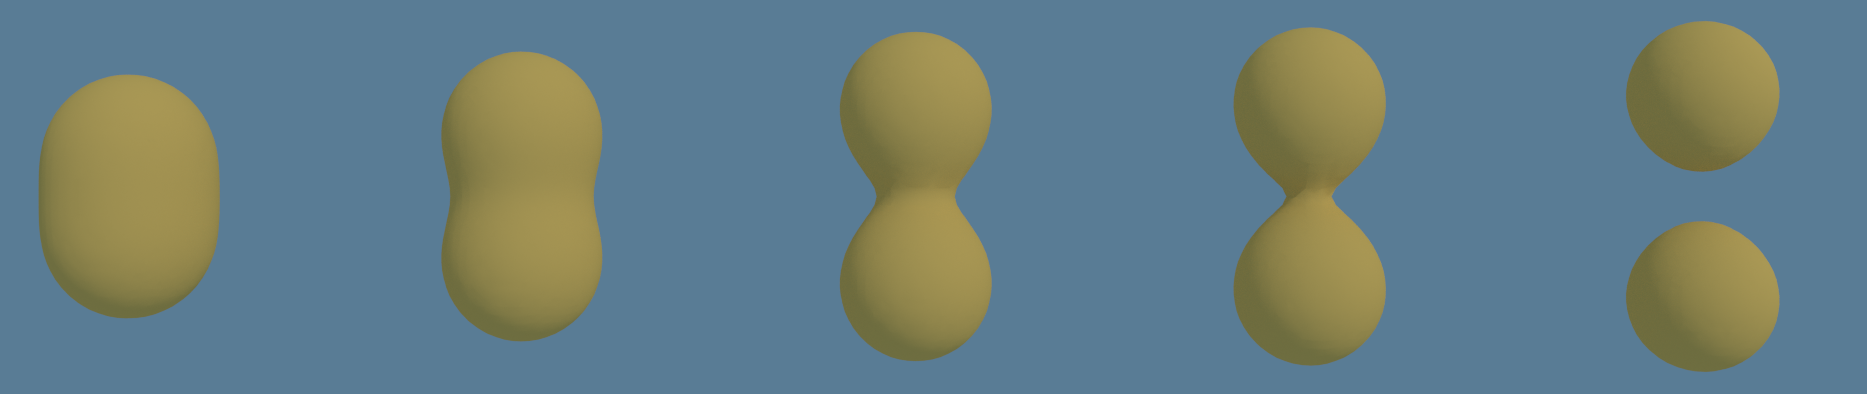
\includegraphics[width=\textwidth]{chapters/project/metaballs.png}
  \end{center}
  \caption{Two metaballs at various distances showing how they are ,,melitng''
    together when getting closer to each other. Geometry was generated with
    \emph{mcblob} program and final image was rendered with Blender 2.68 with
    Cycles renderer. Input file for mcblob that generates this is included with the thesis
      in \texttt{fig\_metaballs.in} file in kartsgen examples.
  }
  \label{fig:metaballs}
\end{figure}


\subsection{Overview}
Both blobber and mcblob are implemented in C++ language with latest C++11
version of the standard. Build system used to compile the code is \emph{CMake}\footnote{Cross--platform make}
-- meta build system that can generate native projects for various IDEs\footnote{Integrated Development Environment}
andactual build systems. Executables use \emph{Boost Program Options} library
for parsing command line arguments and providing help.

Karstgen uses unit testing framework \emph{Google~Test}\footnote{\url{http://code.google.com/p/googletest/}}.
Documentation is automatically generated from sources with Doxygen
tool.


\subsection{Blobber}

For vector data structuers blobber uses \emph{GLM}\footnote{\url{http://glm.g-truc.net/0.9.4/index.html}}
-- a mathematical library that resembles GLSL\footnote{OpenGL Shading Language}.

It reads information about diameters of fractures in fractures network
and places blobs along these fractures with diameters roughly the same as of
these fractures.

Blobber works on data structure named \texttt{DataPoint}:

\begin{lstlisting}
struct DataPoint
{
  	int x, y, z;
	float midDiam;
	std::vector<float> xData;
	std::vector<float> yData;
	std::vector<float> zData;
};
\end{lstlisting}

This structure can describe three fractures originating in index $(x,y,z)$ in
the fracture net and going along each axe in ascending direction. Each fracture
is described as a vector of uniformly distributed diameters. If there is only
one diameter in a vector it is assumed that the fraction it represens has the
same diameter along its whole length. When no diameters are present in some
vector, it is assumed that there is no fracture in this direction.
Additional field \texttt{midDiam} is a diameter of blob that should be placed in
the intersection of the three fractures.

\begin{figure}[hb]
  \begin{center}
    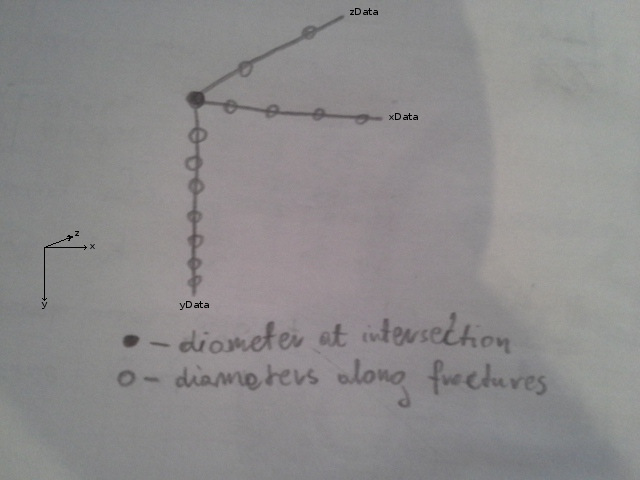
\includegraphics[width=0.7\textwidth]{chapters/project/datapoint.jpg}
  \end{center}
  \caption{Graphical representation of \texttt{dataPoint} -- a basic structure that
blobber works on}
  \label{fig:datapoint}
\end{figure}

Data points are packed into a structure representing whole fracture network
called \texttt{FractureNet}:
\begin{lstlisting}[label={lst:fracturenet},escapeinside={@}{@}]
struct FractureNet
{
	//size of net in number of dataPoints
	int x; int y; int z;
	
	//length of single fracture in each direction
	float xLen; float yLen; float zLen;
	
	std::map<std::tuple<int, int, int>, DataPoint> dataPoints;
};
\end{lstlisting}

Since fracture net is usually quite sparse, dictionary structure\footnote{\texttt{std::map} from C++'s Standard Template Library}
is used to store data points instead of array or vector. Keys in this dictionary
are tuples containing 3D index in a fracture net. This way, given one data point
it is easy to find its neighbours.

\subsubsection{Placement of blobs}

Blobber works on one data point at a time through \texttt{blobs\-From\-Data\-Point()}
function. First, one point is placed in the intersection of the axes with
diameter equal to \texttt{mid\-Point\-Diam}. Then, vector for each non--empty
axe is processed by \texttt{blobsOnVector()} function. Besides the vector of
diameters, this function takes \texttt{midPointDiam} of the data point, and optionally
\texttt{nextDpMidDiam} which is \texttt{midPointDiam} of the next data point
along this axis if such data point exists. Fast lookup of next data point
is possible thanks to dictionary storage of data points. If there is no neighbour data
point at the end of the axis, \texttt{nextDpMidDiam} is considered to be 0.\todo{test if this makes sense}

\begin{figure}[htb]
  \begin{center}
    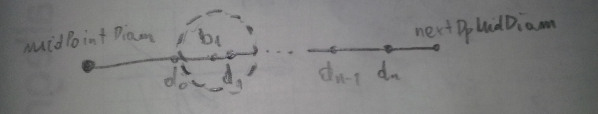
\includegraphics[width=\textwidth]{chapters/project/placement.jpg}
  \end{center}
  \caption{Blobs are placed along fracture defined as set of diameters
    $(d_0,d_1,\cdots,d_{n-1})$. In this example diameter of blob $b_1$ will be a
    linear interpolation of diameters $d_0$ and $d_1$ proportional to distance
    from these diameters.}
  \label{fig:placement}
\end{figure}

Function \texttt{blobsOnVector()} places blobs on the fracture line until
it's fully covered. Diameters of blobs are determined in a way described
in \autoref{fig:placement}.

Format of the input to blobber is described in generated documentation:
\begin{lstlisting}[language=bash,numbers=none]
\doc\blobber\html\index.html
\end{lstlisting}

Output format is the same as input format of mcblob program and is described in
its help:
\begin{lstlisting}[language=bash,numbers=none]
./mcblob --help
\end{lstlisting}

\subsection{Mcblob}
\label{sub:mcblob}

Mcblob uses OpenCL (\autoref{chap:cl}) to calculate density function from
list of blobs provided in input, generates polygon mesh of isosurface
definded by this function using Marching Cubes algorithm (\autoref{chap:marchingcubes})
accelerated with OpenCL and saves results to file in one of two formats.

Bounds of 3D space within which geometry will be generated is defined in input.
It's divided into blocks which are worked on one at a time. For each block,
density function is calculated from blobs, followed by generating geometry.

Finally, when geometry from all blocks is calculated, mcblob writes output to
disk in one of two supported formats.

\subsubsection{Calculating density function}

Each block of voxels is kept by mcblob in a class called \texttt{Grid}. It
contains values of density function on the vertices of the cubes in a block.
These values are stored as one--dimensional array, that is transferable between host and
device memory. If number of voxels on $x$, $y$ and $z$ axes is $v_x$, $v_y$
and $v_z$ respectively, \texttt{Grid} will store 1D array
of \texttt{float4} values $(v_x+1)\times(v_y+1)\times(v_z+1)$ elements long.

\begin{figure}[tb]
  \begin{center}
    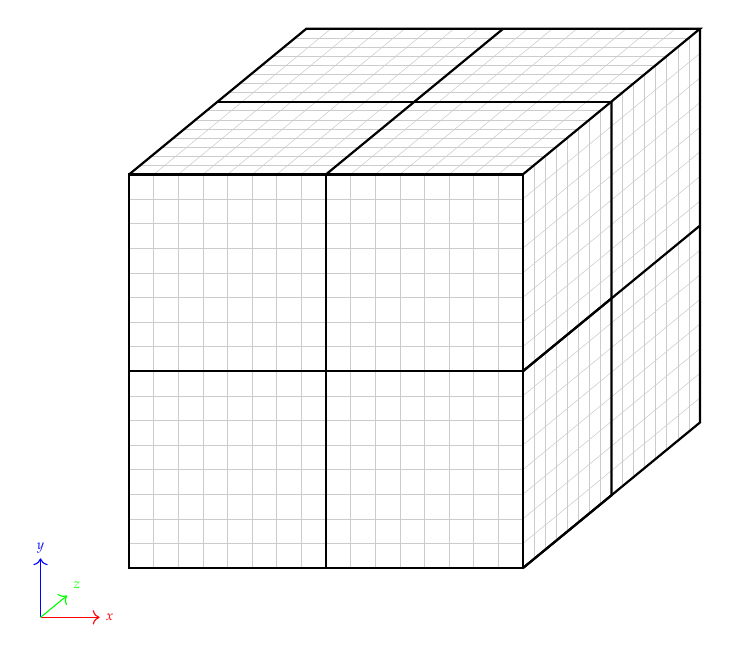
\begin{tikzpicture}[z={(-0.45cm,-0.37cm)}, scale=2.5]

\tikzstyle{inner} = [gray!40!white,very thin]
%front face vertical
\foreach \x in {1,2,3,4,5,6,7,9,10,11,12,13,14,15}
  \draw[inner] (\x/8,0) -- (\x/8,2);
%front face horizontal
\foreach \x in {1,2,3,4,5,6,7,9,10,11,12,13,14,15}
  \draw[inner] (0,\x/8) -- (2,\x/8);

%rigt face vertical
\foreach \x in {1,2,3,4,5,6,7,9,10,11,12,13,14,15}
  \draw[inner] (2,0,-\x/8) -- (2,2,-\x/8);
%rigth face horizontal
\foreach \x in {1,2,3,4,5,6,7,9,10,11,12,13,14,15}
  \draw[inner] (2,\x/8,0) -- (2,\x/8,-2);

%top face front to back
\foreach \x in {1,2,3,4,5,6,7,9,10,11,12,13,14,15}
  \draw[inner] (\x/8,2,0) -- (\x/8,2,-2);
%top face left to rigth
\foreach \x in {1,2,3,4,5,6,7,9,10,11,12,13,14,15}
  \draw[inner] (0,2,-\x/8) -- (2,2,-\x/8);


\draw[thick] (0,0) rectangle (1,1);
\draw[thick] (1,0) rectangle (2,1);
\draw[thick] (0,1) rectangle (1,2);
\draw[thick] (1,1) rectangle (2,2);

\draw[thick] (2,1) -- (2,1,-1) -- (2,2,-1);
\draw[thick] (2,1) -- (2,1,-2) -- (2,2,-2);
\draw[thick] (2,0) -- (2,0,-1) -- (2,1,-1);
\draw[thick] (2,0) -- (2,0,-2) -- (2,1,-2);

\draw[thick] (1,2) -- (1,2,-2);
\draw[thick] (0,2,-1) -- (2,2,-1);

\draw[thick] (0,2) -- (0,2,-2) -- (2,2,-2) -- (2,2);

\draw[red,->] (-0.45,-0.25) -> (-0.15,-0.25) ;
\draw[red] (-0.1, -0.25) node[font=\tiny] {$x$};

\draw[blue,->] (-0.45,-0.25) -> (-0.45, 0.05);
\draw[blue] (-0.45, 0.1) node[font=\tiny] {$y$};


\draw[green,->] (-0.45,-0.25) -> (-0.45, -0.25, -0.3);
\draw[green] (-0.40, -0.20, -0.3) node[font=\tiny] {$z$};

\end{tikzpicture}
  \end{center}
  \caption{In this configuration, domain is divided into $2\times2\times2=8$
  grids, and each one of them consists of $8\times8\times8=512$ voxels totalling
 $512\times8=4096$ voxels.}
  \label{fig:grid}
\end{figure}

Four floats are kept for each vertex instead of one to facilitate computation of
normal vectors. In case of \texttt{Grid} components $x$, $y$ and
$z$ store density function values in positions shifted by small value along
respective axes and $w$ component stores value at the vertex itself.

Density function of a set of blobs is calculated by method:
\begin{lstlisting}[numbers=none]
Blob::runBlob()
\end{lstlisting}
that adds array of blobs to the grid according to \autoref{eq:metaballdensity}.
For better performance, this method utilizes constant memory. Device is queried
for size of constant memory via \texttt{cl::Device::getInfo()}. As
mentioned in \autoref{chap:cl} constant memory is efficient for data that is
simultaneously accessed by many threads. In case of \texttt{Blob} program,
every thread iterates over all blobs. If size of blob data exceeds constant
memory size, input is divided into packets that are within the limit, and kernel
is simply invoked multiple times, until all blobs are processed.

This method of implementation was inspired by MRI\footnote{Magnetic resonance imaging}
reconstruction program for CUDA described in \cite[in chapter~8]{Kirk:2010:PMP:1841511}.

\subsubsection{Generating geometry}

When density function of all blobs is calculated for a single grid, such grid
is submitted to:
\begin{lstlisting}[language=bash,numbers=none]
MarchingCubes::compute()
\end{lstlisting}
method that runs OpenCL--powered
Marching Cubes implementation (see \autoref{sec:mcgpu}). Once the geometry for
all blocks is generated, it's passed to one of two exporter functions that write
the results to disk in format selected by the user. Wavefront OBJ output can be
imported by virtually every 3D graphics software and AVR can be read by aforementioned
Vorticity game engine.

\subsection{Using \texttt{blobber} and \texttt{mcblob} together}

Blobber and mcblob are naturally fit to be executed in shell via piping. To
run karstgen with provided examples, go to folder where it was compiled and
type:
\begin{lstlisting}[language=bash,numbers=none]
cat [input] | ./blobber | ./mcblob -o out.obj
\end{lstlisting}
Where \texttt{[input]} is path to a file with description of fracture net.
Examples are located in \texttt{examples\\blobber}.
This will generate \texttt{out.obj} file that can be imported to 3D graphics
program.

To randomly disturb positions of blobs by 15\% and sizes by 10\% of their
diameter, invoke karstgen in the following manner:
\begin{lstlisting}[language=bash,numbers=none]
cat [input] | ./blobber -p 15 -s 10 | ./mcblob -o out.obj
\end{lstlisting}

\section{Example outputs}
Below are screenshots of outputs of karstgen with references to input files used
to produce them.

\begin{figure}[htb]
  \begin{center}
    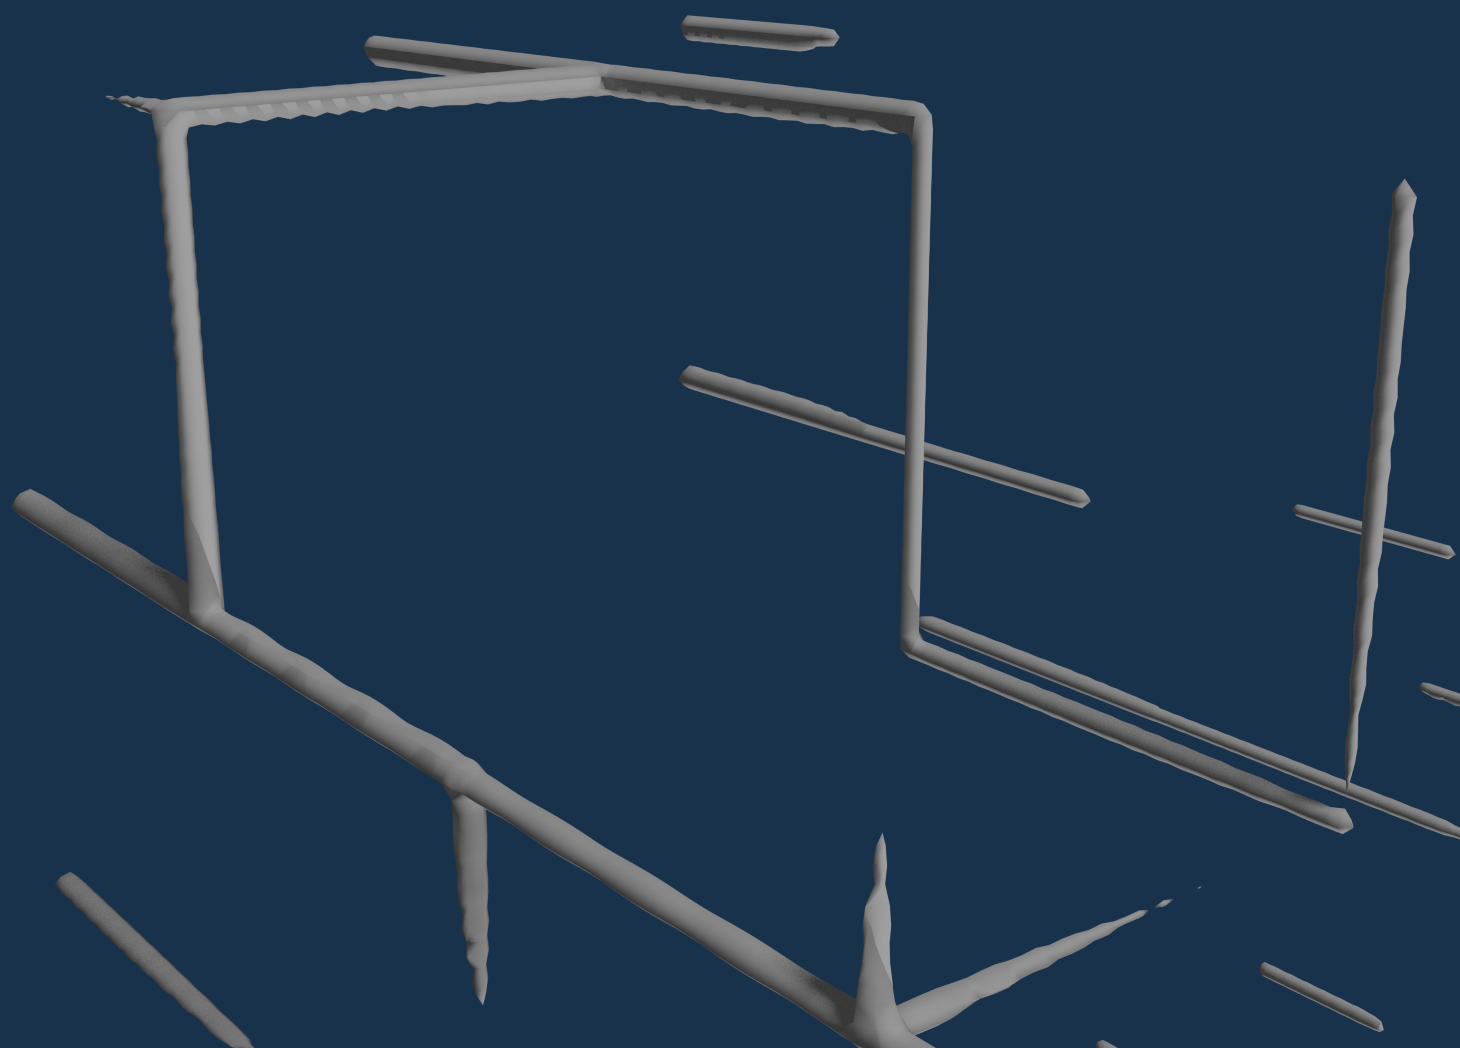
\includegraphics[width=\textwidth]{chapters/project/hiller_result.png}
  \end{center}
  \caption{Rendering of result of simulation generated by KARSTAQUIFER tool \parencite{Kaufmann200962}.
  Input data file courtesy of Mr Thomas Hiller PhD from Free University of Berlin.
  Available in file \texttt{examples\textbackslash blobber\textbackslash hiller.in}. Be advised, that
  due to very large domain, computations done by karstgen may take several hours.
  Figure rendered with Blender renderer.}
  \label{fig:hillershot}
\end{figure}

\begin{figure}[htb]
  \begin{center}
    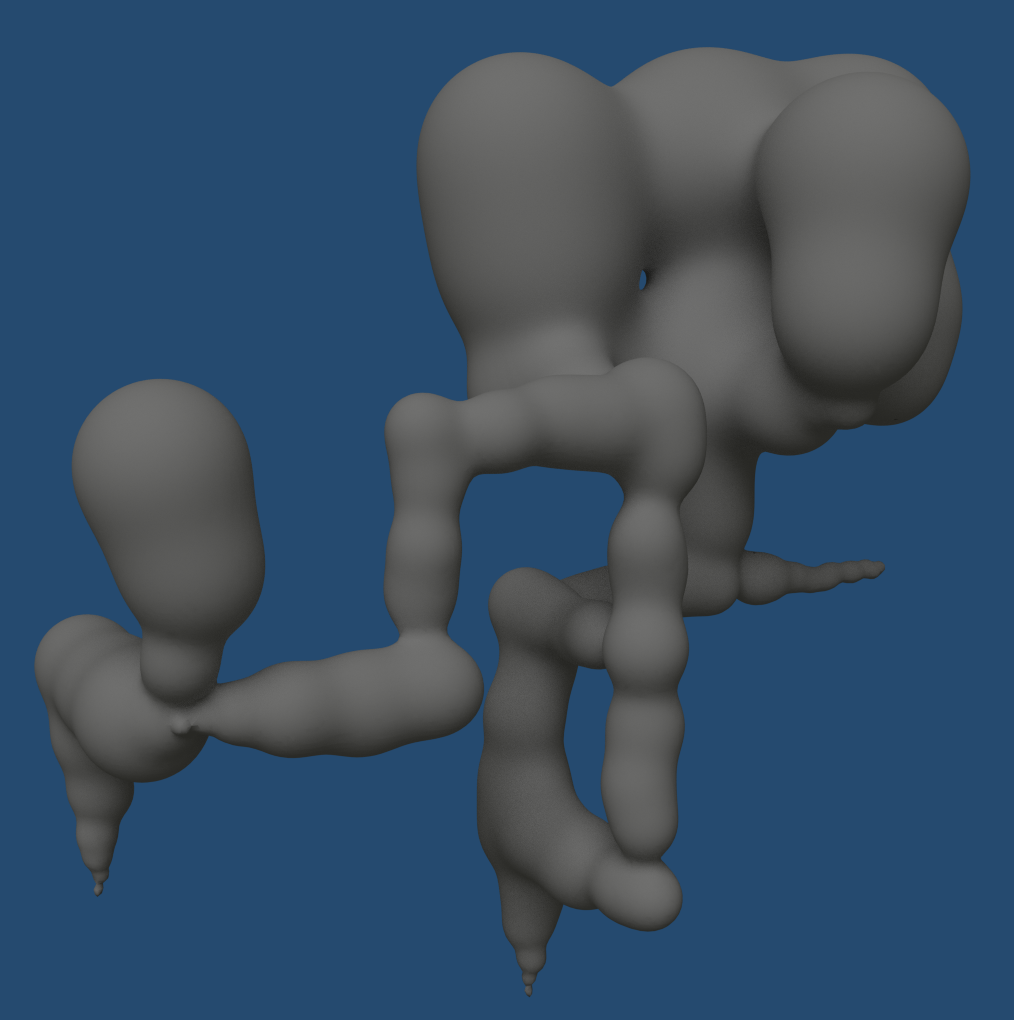
\includegraphics[width=\textwidth]{chapters/project/synthetic.png}
  \end{center}
  \caption{Render of synthetic blobber input file created by author. Rendered
    with Blender Cycles renderer. Input file available at \texttt{examples\textbackslash blobber\textbackslash synthetic.in}}
  \label{fig:synthetic}
\end{figure}

\begin{figure}[htb]
  \begin{center}
    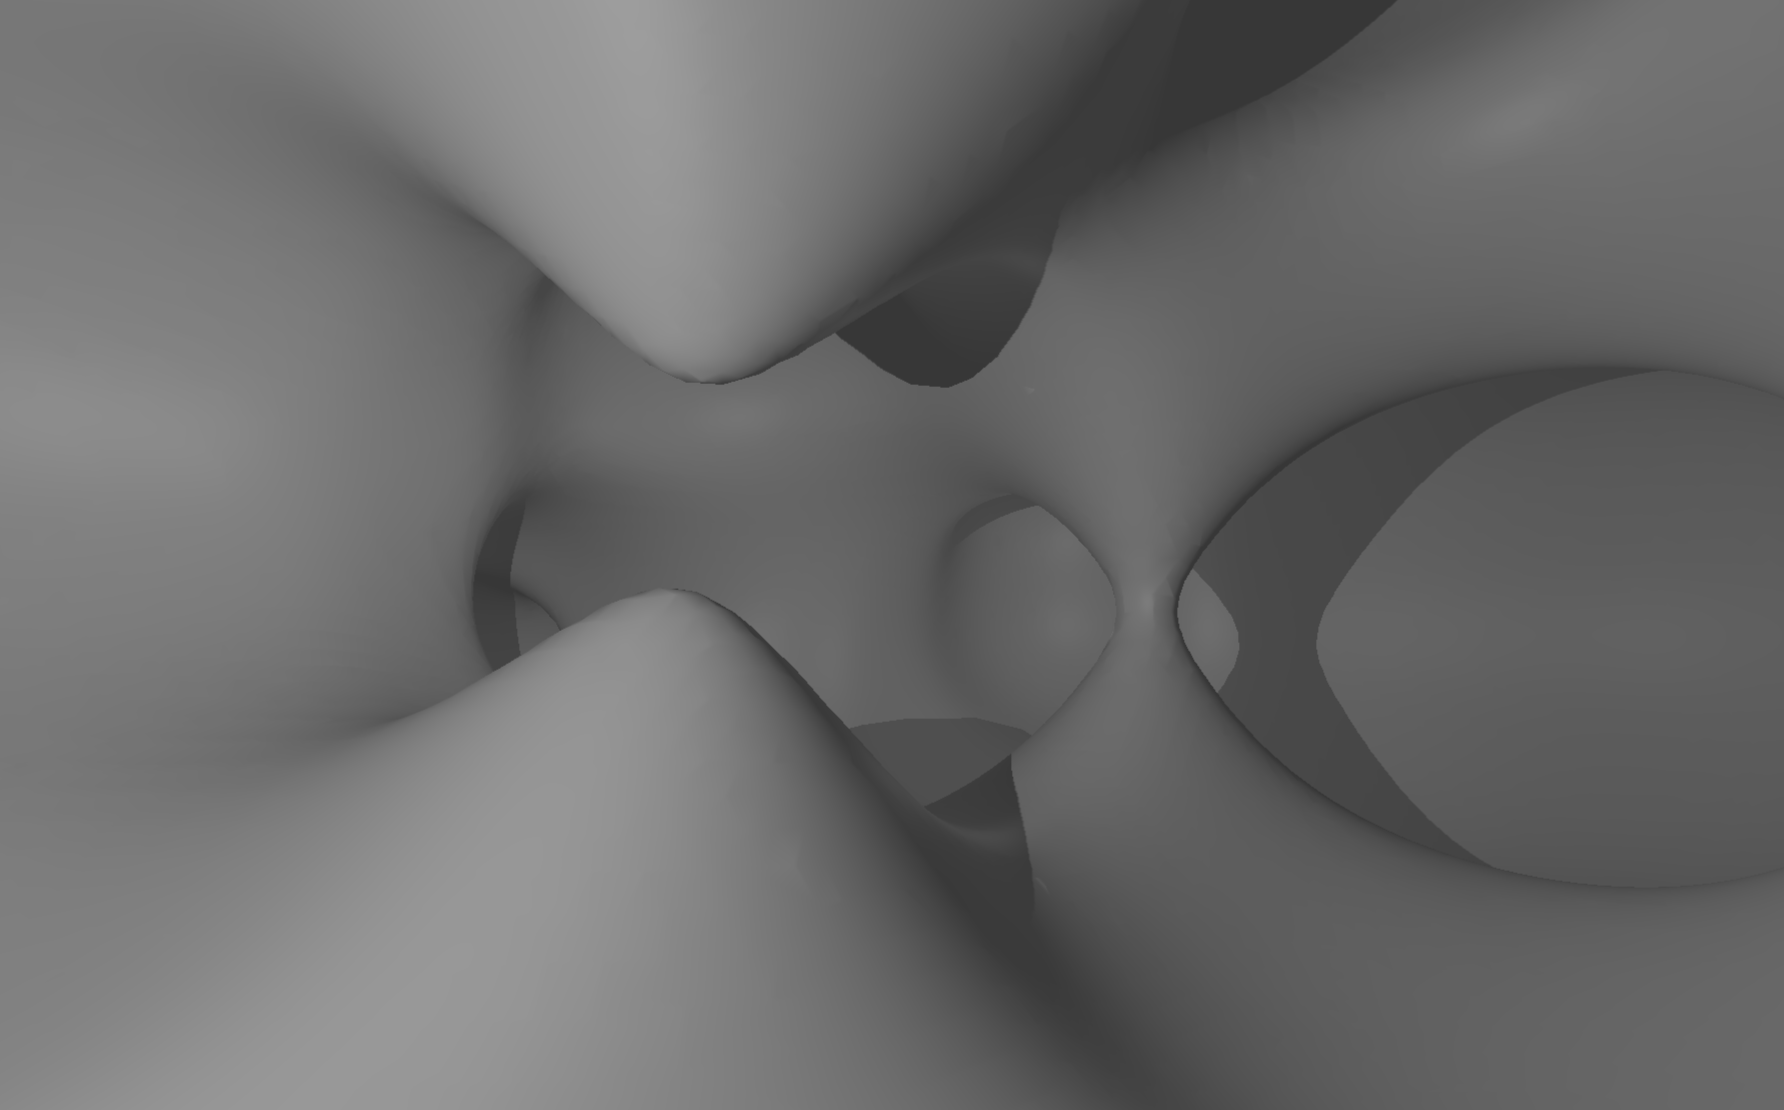
\includegraphics[width=\textwidth]{chapters/project/interior.png}
  \end{center}
  \caption{Interior of the cave generated for \autoref{fig:synthetic}. Rendered with
Blender renderer.}
  \label{fig:interior}
\end{figure}

\chapter{Conclusions and further work}
\label{chap:furtherwork}


\printbibliography
\end{document}
